\PassOptionsToPackage{dvipsnames,table}{xcolor}
\documentclass[10pt]{beamer}
\usetheme[options]{Madrid} 

\usepackage{../../latex/Cours}



\begin{document}
	
	\input{\detokenize{../../latex/MacrosCours.tex}}
\setcounter{numchap}{7}
\newcommand{\DB}{\dnum  Exercice 1 : SQL}
\newcommand{\Arbre}{\dnum  Exercice 2 : Arbres binaires équilibrés}

\pythonmode

\lstset{language=python,numbers=left, tabsize=2, frame=single, breaklines=true, basicstyle=\ttfamily,
	numberstyle=\tiny\ttfamily, framexleftmargin=0mm, backgroundcolor=\color{grispale}, xleftmargin=12mm}

 \title{Epreuve écrite type BAC}
 \subtitle{20 février 2023}

  \frame{\titlepage}

% Définition langage de programmation


\begin{frame}
	\mframe{\DB}
	\begin{exampleblock}{Question 1}
    La table \textcolor{blue}{\sc Articles} utilise des clés étrangères des tables \textcolor{blue}{\sc Auteurs} et \textcolor{blue}{\sc Themes}. Si ces dernières sont vides, il n'est pas possible de lier les valeurs et donc on ne peut pas insérer de valeurs.
	\end{exampleblock}
	\onslide<2->\begin{exampleblock}{Question 2}
 On saisit \textcolor{blue}{\sc INSERT INTO} Traitements (article, theme) \textcolor{blue}{\sc VALUES}  (2, 4)
\end{exampleblock}
	\onslide<3->\begin{exampleblock}{Question 3}
	On saisit \textcolor{blue}{\sc UPDATE} Auteurs \textcolor{blue}{\sc SET} nom="Jèraus" \textcolor{blue}{\sc WHERE} idAuteur = 2
\end{exampleblock}

\end{frame}


\begin{frame}
	\mframe{\DB}
	\begin{exampleblock}{Question 4.a}
        Le titre des articles parus après le $1^{er}$ janvier 2022 inclus :\\

 \textcolor{blue}{\sc SELECT} titre \\
 \textcolor{blue}{\sc FROM} Articles\\
 \textcolor{blue}{\sc WHERE}  dateParution >= 20220101
\end{exampleblock}
	\onslide<2->\begin{exampleblock}{Question 4.b}
        Le titre des articles écrits par l'auteur Étienne Zola :\\

 \textcolor{blue}{\sc SELECT} titre \\ 
 \textcolor{blue}{\sc FROM} Articles \\
 \textcolor{blue}{\sc WHERE} auteur = 3
\end{exampleblock}
	
\end{frame}

\begin{frame}
	\mframe{\DB}
	\begin{exampleblock}{Question 4.a}
        Le nombre d'articles écrits par l'auteur Jacques Pulitzer (présent dans la table  \textcolor{blue}{\sc Auteurs} mais on ne connaît pas son  \textcolor{blue}{\sc idAuteur}) : \\

 \textcolor{blue}{\sc SELECT} count(*) \\
 \textcolor{blue}{\sc FROM} Articles \\
 \textcolor{blue}{\sc JOIN} auteurs  \textcolor{blue}{\sc ON} Articles.auteur = Auteurs.idAuteur \\
 \textcolor{blue}{\sc WHERE} nom  \textcolor{blue}{\sc LIKE} "Pulitzer"  \textcolor{blue}{\sc AND} prenom  \textcolor{blue}{\sc LIKE} "Jacques"
	\end{exampleblock}
	\onslide<2->\begin{exampleblock}{Question 4.b}
Les dates de parution des articles traitant du thème \og Sport \fg\ :\\

\textcolor{blue}{\sc SELECT} dateParution \\
\textcolor{blue}{\sc  FROM} Articles \\
\textcolor{blue}{\sc JOIN} Traitements \textcolor{blue}{\sc ON} Articles.idArticle = Traitements.article \\
\textcolor{blue}{\sc JOIN} Themes \textcolor{blue}{\sc ON} Traitements.theme = Themes.idTheme  \\
\textcolor{blue}{\sc WHERE} Themes.themes \textcolor{blue}{\sc LIKE} "Sport" \\
.
	\end{exampleblock}
\end{frame}

\begin{frame}
	\mframe{\Arbre}
	\begin{exampleblock}{Question A.1.a}
	 On obtient :
	
	\begin{figure}[H]
		\begin{center}
			\footnotesize{
				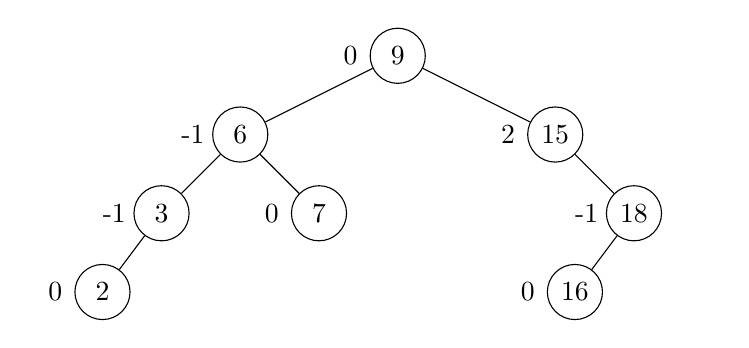
\begin{tikzpicture}[level distance=1cm,level 1/.style={sibling distance=4cm},
					level 2/.style={sibling distance=2cm},
					level 3/.style={sibling distance=1.5cm}]
					\tikzstyle{every node}=[draw, circle, minimum size=7mm, inner sep=1mm]
					
					\node at (0,0) (9) {9} []
					child {node (6) {6}
						child {node (3) {3}
							child {node (2) {2}}
							child {node[draw=none] {} edge from parent [draw=none]}
						}
						child {node (7) {7}
						}
					}
					child {node (15) {15}
						child {node[draw=none] {} edge from parent [draw=none]}
						child {node (18) {18}
							child {node (16) {16}}
							child {node[draw=none] {} edge from parent [draw=none]}
						}
					};
					
					\node[draw=none, xshift=-6mm, yshift=0mm] at (9) {0};
					\node[draw=none, xshift=-6mm, yshift=0mm] at (6) {-1};
					\node[draw=none, xshift=-6mm, yshift=0mm] at (15) {2};
					\node[draw=none, xshift=-6mm, yshift=0mm] at (3) {-1};
					\node[draw=none, xshift=-6mm, yshift=0mm] at (7) {0};
					\node[draw=none, xshift=-6mm, yshift=0mm] at (18) {-1};
					\node[draw=none, xshift=-6mm, yshift=0mm] at (2) {0};
					\node[draw=none, xshift=-6mm, yshift=0mm] at (16) {0};
					
				\end{tikzpicture}
			}
		\end{center}
	\end{figure}
	\end{exampleblock}
	\onslide<2->\begin{exampleblock}{Question A.1.b}
 Cet arbre n'est pas équilibré car le nœud de valeur 15 a une balance de 2.
		\end{exampleblock}
\end{frame}


\begin{frame}
	\mframe{\Arbre}
	\begin{exampleblock}{Question A.2.a}
	  On obtient \textcolor{red}{\sc [0, 45, 40, 48, 17, 43, 46, 49, 14, 19]}
	\end{exampleblock}
	\onslide<2->\begin{exampleblock}{Question A.2.b}
	      On obtient :
	
	\begin{figure}[H]
		\begin{center}
			\footnotesize{
				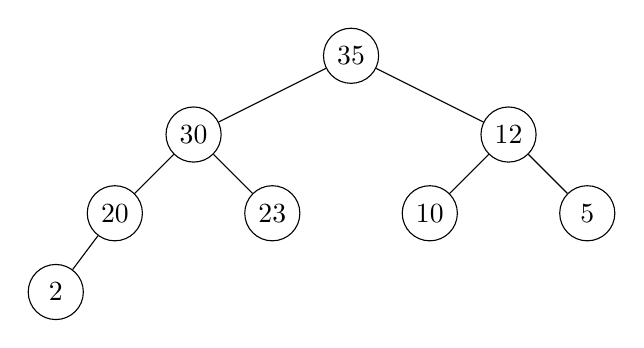
\begin{tikzpicture}[level distance=1cm,level 1/.style={sibling distance=4cm},
					level 2/.style={sibling distance=2cm},
					level 3/.style={sibling distance=1.5cm}]
					\tikzstyle{every node}=[draw, circle, minimum size=7mm, inner sep=1mm]
					
					\node at (0,0) {35} []
					child {node {30}
						child {node {20}
							child {node {2}}
							child {node[draw=none] {} edge from parent [draw=none]}
						}
						child {node {23}}
					}
					child {node {12}
						child{node {10}}
						child{node {5}}
					};
				\end{tikzpicture}
			}
		\end{center}
	\end{figure}   
	\end{exampleblock}
\end{frame}


\begin{frame}
	\mframe{\Arbre}
	\begin{exampleblock}{Question A.3.a}
	  \textcolor{red}{f(arbre, 1)} renvoie 3. En effet, si l'arbre est vide ou si la valeur de sa racine est \textcolor{red}{\sc None}, on renvoie $0$. Dans le cas contraire, on renvoie
	$1$ plus de maximum des résultats des sous-arbres gauches et droits (indices \textcolor{red}{2*i} et \textcolor{red}{2*i+1}). On calcule ainsi la hauteur de l'arbre.
	\end{exampleblock}
	\onslide<2->\begin{exampleblock}{Question A.3.b}
      La fonction \textcolor{red}{f} permet de calculer la hauteur d'un arbre.
	\end{exampleblock}
\end{frame}

\begin{frame}[fragile]
	\mframe{\Arbre}
	\begin{block}{Question A.4}
		\begin{lstlisting}
def estEquilibre(arbre: list, i : int) -> bool:
   if i >= len(arbre) or arbre[i] is None:
        return True
    else:
        balance = f(arbre, 2*i+1) - f(arbre, 2*i)
        reponse = balance in [-1, 0, 1]
        return reponse and estEquilibre(arbre,2*i) and estEquilibre(arbre, 2*i+1)
		\end{lstlisting}
	\end{block}
\end{frame}

\begin{frame}
	\mframe{\Arbre}
	\begin{exampleblock}{Question B.1}

      \begin{figure}[!ht]
        \centering
        \footnotesize{

          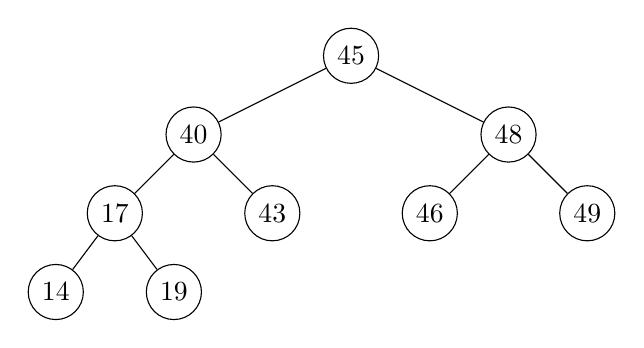
\begin{tikzpicture}[level distance=1cm,level 1/.style={sibling distance=4cm},
              level 2/.style={sibling distance=2cm},
              level 3/.style={sibling distance=1.5cm}]
            \tikzstyle{every node}=[draw, circle, minimum size=7mm, inner sep=1mm]

            \node {45}
            child {node {40}
                child {node {17} {
                        child {node {14}}
                        child {node {19}}
                      }}
                child {node {43}}
              }
            child {node {48}
                child {node {46}}
                child {node {49}}
              };
          \end{tikzpicture}
        }
      \end{figure}
    \begin{itemize}[label=\textbullet]
      \item<1-> Parcours \textit{préfixe} : 45, 40, 17, 14, 19, 43, 48, 46, 49
      \item<2-> Parcours \textit{infixe} : 14, 17, 19, 40, 43, 45, 46, 48, 49 
      \item<3-> Parcours \textit{suffixe} : 14, 19, 17, 43, 40, 46, 49, 48, 45
    \end{itemize}
	\end{exampleblock}
\end{frame}

\begin{frame}[fragile]
	\mframe{\Arbre}
	\begin{exampleblock}{Question B.2}
    On obtient :

      \begin{figure}[H]
        \begin{center}
          \footnotesize{
            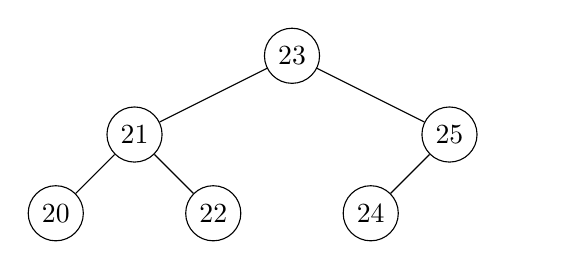
\begin{tikzpicture}[level distance=1cm,level 1/.style={sibling distance=4cm},
                level 2/.style={sibling distance=2cm},
                level 3/.style={sibling distance=1.5cm}]
              \tikzstyle{every node}=[draw, circle, minimum size=7mm, inner sep=1mm]
    
              \node at (0,0) {23}
                child {node {21}
                  child {node {20}}
                  child {node {22}}
                }
                child {node {25}
                  child {node {24}}
                  child {node[draw=none] {} edge from parent [draw=none]}
                };
            \end{tikzpicture}
          }
        \end{center}
      \end{figure}  
	\end{exampleblock}
\end{frame}


\begin{frame}[fragile]
	\mframe{\Arbre}
	\begin{exampleblock}{Question B.3}
			\begin{lstlisting}
def infixe(arbre: list) -> list:
    pile = []
    visites = []
    n = 1
    repetition = True
    while repetition :
        while n < len(arbre) and arbre[n] is not None :
            pile.append(n)
            n = 2*n
        if len(pile) == 0 :
            repetition = False
        else :
            n = pile.pop()
            visites.append(arbre[n])
            n = 2*n+1
    return visites
   		\end{lstlisting}
	\end{exampleblock}
\end{frame}


\begin{frame}[fragile]
	\mframe{\Arbre}
	\begin{exampleblock}{Question B.4}
			\begin{lstlisting}
def construitABR(i, ordre):
#Ajoute la valeur None à la liste nouveau jusqu'à ce qu'elle soit de longueur i+1
    while len(nouveau) <= i:
        nouveau.append(None)
# Donne la valeur du milieu de ordre à nouveau[i]
    i_milieu = len(ordre)//2
    nouveau[i] = ordre[i_milieu]
# Détermine la moitié gauche de ordre
    gauche = ordre[:i_milieu]
# Si celle-ci est non-vide, appelle construireABR(2*i, moitié gauche de ordre)
    if len(gauche) > 0:
        construitABR(2*i, gauche)
    droite = ordre[(i_milieu+1):]
    if len(droite) > 0:
        construitABR(2*i+1, droite)
   		\end{lstlisting}
	\end{exampleblock}
\end{frame}

\end{document}